 \subsection{Clone Manager} 
\label{sec:CloneManager}

%\subsubsection{How does cloning work?}
%\label{sec:cloning}

%While the focus of our work is not to support container migration, or to make changes to the hypervisor, we need to tweak the way typical hypervisors offer live migration for our purposes.
%Before moving further we wish to clarify that instead of the standard live migration supported by hypervisors, \parikshan requires a cloning functionality. 
%In contrast with live migration, where a container is copied to a target destination, and then the original container is destroyed, the cloning process requires both containers to be actively running, and be still attached to the original network.
%This cloning requires modification in both how compute migration is handled, and especially how the network migration is handled. 

Before describing cloning in our context, let us first review some details about live migration~\cite{livemigration}. 
Live migration refers to the process of moving a running virtual machine, or container from one server to another, without disconnecting any client or process running within the machine. 
%It is supported by most well known Hypervisors (VMware, VirtualBox, Xen, Qemu, KVM).
% with different amounts of efficiency.
%There are several different mechanisms for migration, some of which require a short suspend time, while others are able to seamlessly transfer without any noticeable down-time by the user.
In general, this involves the following steps: 
(1) A pre-copy \texttt{rsync}, whereby the underlying hypervisor copies all the memory pages from the source node to the destination node. 
(2) Once the pre-copy phase is finished, the VM is temporarily suspended, and all pages which were modified are transferred to the target node. 
%Live migration needs two rsync's, the first one moves most of the data while the container is still up and running, and the second one moves the changes made during the time period between the first rsync run and the container pause.
The second step can be done in multiple iterations to avoid a long suspend time, in-case the memory pages have significantly changed after the first rsync. 
%\footnote{Network migration is managed by the IAAS which publishes the same MAC address for the copied VM. 
%Since the identity of the target container remains the same, the IAAS is able to give it same IP Address, and network traffic is rerouted after the identity is published in the network}.
%To reduce the down-time memory pages are transferred probabiliticly based on priority, and incase a page is not found a network fault is generated which executes a fetch from the original VM.

In contrast, live migration where the original container is destroyed, the ``Live Cloning'' process used in \parikshan requires both containers to be actively running, and be still attached to the original network.
%Instead of Live Migration, in Live Cloning, we do not delete the source container, rather we allow the container to keep executing in both production and test locations.
The challenge here is to manage two containers with the same identities in the network and application domain. 
This is important, as the operating system and the application processes running in it may be configured with the IP address, which cannot be changed on the fly.
Hence, the same network identifier should map to two separate addresses, and have communication with no problems or slowdowns.
%Test and production containers can be allocated in various schemes: we call these schemes \textit{modes}. 

We now describe two modes (see Figure~\ref{fig:modesCloning}) in which cloning has been applied, followed by the algorithm for live cloning:

\begin{figure}[t]
  \begin{center}
    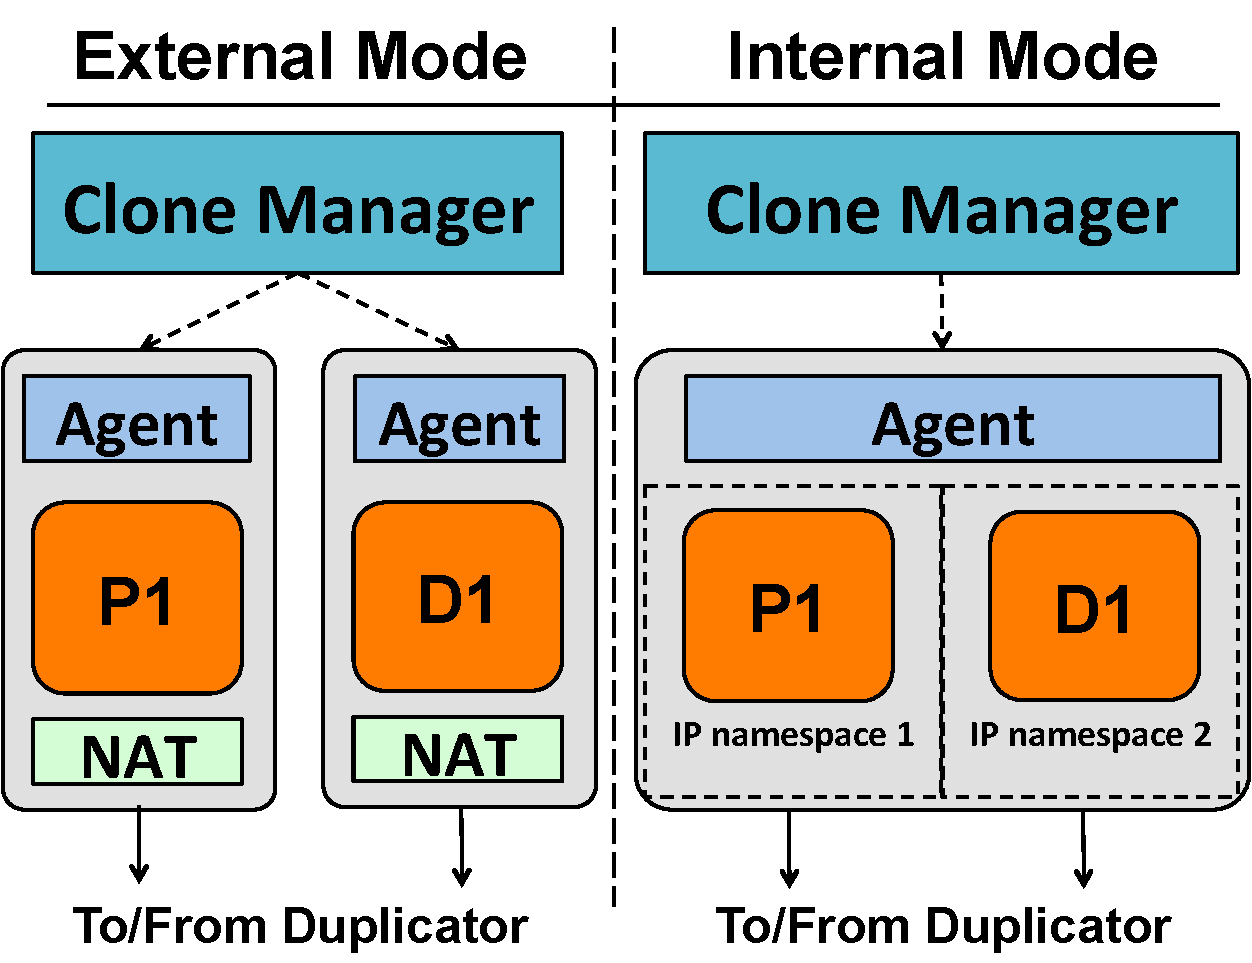
\includegraphics[width=0.45\textwidth]{figs/ModesCloning.pdf}
    \caption{External and Internal Mode for live cloning: P1 is the production container, and D1 is the debug container, the clone manager interacts with an agent which has drivers to implement live cloning.}
    \label{fig:modesCloning}
  \end{center}
\end{figure}

%\begin{itemize}[leftmargin=*,topsep=0pt,itemsep=-1ex,partopsep=1ex,parsep=1ex]

%\item 
\noindent
\textbf{\textit{Internal Mode}}: In this mode we allocate the production and debug containers to the same host node. 
This would mean less suspend time, as the production container can be locally cloned (instead of streaming over the network). 
Additionally, it is more cost-effective since the number of servers remain the same.
On the other hand, co-hosting the debug and production containers could potentially have an adverse effect on the performance of the production container because of resource contention.

To manage network identities, we encapsulate each container in separate network namespaces.
This allows both the containers, to have the same IP address, although in separate interfaces.
%In the internal mode, network identity of the containers is encapsulated within different network namespaces.
%As we can see in Figure~\ref{fig:modesCloning}, the production container P1 and debug container T1 are both hosted within the same physical host, and with the same IP address.
%However, their network is encapsulated within different network namespaces to sandbox them.
The duplicator is then able to communicate to both these containers with no networking conflict.

%\item 
\noindent
\textbf{\textit{External Mode}}: In this mode we provision an extra server as the host of our debug-container (this server can host more than one debug-container). 
While this mechanism can have a higher overhead in terms of suspend time (dependent on workload), and requires provisioning an extra host-node, the advantage of this mechanism is that once cloned, the debug-container is totally separate and will not impact the performance of the production-container.
We believe that external mode will be more practical in comparison to internal mode, as cloning is likely to be transient, and high network bandwidth between physical hosts can offset the slowdown in cloning performance. 
%It is often more important to not impact user experience. 
%However, when running in the internal-mode, the test could potentially impact the production run due to co-location in the same host (resource contention etc.).

Network identities in external mode are managed using NAT~\cite{nat} (network address translator) in both host machines. 
Hence both containers can have the same address without any conflict.\footnote{Another additional mode can be \textit{Scaled Mode}: This can be viewed as a variant of the external mode, where we can execute debug analysis in parallel on more than one debug-containers each having it's own cloned connection. This will distribute the instrumentation load and allow us to do more analysis concurrently, without overflowing the buffer. We aim to explore this in the future.}


% the production container P1 and debug container T1 are hosted on two different host machines, and are encapsulated behind a .
%Thus, they each have their own IP addresses in an internal network thereby avoiding any 

%conflict.

%\end{itemize}

%\RestyleAlgo{boxruled}
%\LinesNumbered

%\\ \\
%\noindent \textbf{Implementation}\\
\noindent
\textbf{Algorithm:} 
%The Clone Manager is responsible for creating a live running ``clone'' of the production container and launch it as the test-container. 
%In our current setup cloning is done for each target production environment in the same physical host machine 
%(we can clone to a different physical host as well, however for optimization purposes we have assumed that they will always be in the same local network).
In our current implementation, we are using OpenVZ~\cite{openvz} as our container engine, and leverage OpenVZ tools~\cite{vzctl}~\cite{mirkin2008containers} to support cloning.
% and have modified the migration mechanism in vzctl~\cite{vzctl} to make it work for live cloning instead. 
We tested this out on multiple VM's acting as host nodes for OpenVZ containers. 
To make the cloning easier and faster, we used OpenVZ's \textit{ploop} devices~\cite{ploop} as the container disk layout. 
\textit{Ploop} devices are a variant of disk loopback devices where the entire file system of the container is stored as a single file. 
This allows for easier snapshots/checkpoints, as \textit{ploop} ensures separation of inodes of each container file system.
%The algorithm for live cloning is explained in 
%Algorithm \ref{algCloning} describes the process of live-cloning.

\iffalse
%This was included for USENIX
\begin{algorithm}[ht!]
  \caption{Live cloning algorithm using OpenVZ} 
  \label{algCloning}
  \begin{enumerate}[topsep=0pt,itemsep=-1ex,partopsep=1ex,parsep=1ex]
  \item Safety checks and pre-processing 
%(Checks that a destination server is available via ssh w/o entering a password, and version checking of OpenVZ running in it) 
  \item Synchronize container's file system using rsync utility  
  \item Suspend the production container process
  \item Dump the container and save it to a file on disk
  %\item Start container locally 
  \item Set up port forwarding, packet duplication, and aggregation proxy
  \item During the first synchronization the container is still running. 
Hence some files may be outdated. 
A second rsync is run when the container is suspended to bring both production and debug container at the same state
  \item Transfer dump file and resume both production and debug containers
  \end{enumerate}
\end{algorithm}
\fi

%\begin{example}
Let's imagine we are cloning production container P1 on Host H1 as debug-container D1 on Host H2. 
The initial setup requires certain safety checks and pre-processing to ensure easy cloning. 
These include: ssh-copy-id operation for password-less rsync, checking pre-existing container ID's, version of OpenVZ etc. 
This ensures that H1 and H2 are compatible, and ready for live-cloning.
Next, we run an initial rsync of container P1, from Host H1 to Host H2. 
This step does not require any suspension of P1, and copies the bulk of the container file system to the destination server (H2). 
The next step involves checkpointing, and dumping the process in memory state to a file.
This is what allows the container to be restarted from the same checkpointed state. 
Since the first rsync and the memory dump are non-atomic operations, some of the files in the file system may be outdated.
%However for sanity of the container process, it is important to restart the container from the same file system state as it was when the checkpoint was taken.
We freeze the processes in the production-container, and take a second rsync of the ploop device of P1, to ensure both containers have the same file-system. 
Simultaneously, we setup the networking proxy and aggregation infrastructure to allow for communication from the downstream and upstream servers.
%After this the original container can be restarted.
Next we copy the dump file from step 3, from H1 to H2, and resume both containers.
%\end{example}

The suspend time of cloning depends on the operations happening within the container between step 2 and step 4 (the first and the second rsync), as this will increase the number of dirty pages in the memory, which in turn will impact the amount of memory that needs to be copied during the suspend phase.
In section \ref{sec:performance}, we evaluate the performance of live cloning on some real-world examples and a micro-benchmark of I/O operations. 
%(as mostly the dirty bits at suspend time are those which were not committed to memory and hence need to be transferred).  
%A few iteration of cloning a container back and forth between two OpenVZ instances (on KVM's within the same physical machine), resulted in an average suspend time of 1.8 seconds for the production container.
%( see table \ref{table:clonePerf}).
%add citation for OpenVZ Live Migration performance iteration testbed http://openvz.livejournal.com/47780.html
%This is nearly the same as that of native live migration\cite{openvzLiveMigrationPerf}, and has lesser suspend time for the production container as we do not include the \textit{``copy dump file''}, or the \textit{``undump and resume phase''} for production containers. 
%In section \ref{sec:performance}, we evaluate the performance of live cloning while doing increasing amount of random I/O write operations, as well as with doing page fetches  from web-server running the production container.

%The same amount of resources as the production container are reserved for the test-container. 
%After doing the pre-copy, we do a pause for syncing the two containers, and start them together. 
%Subsequent clone operations are optimized as they only require rsync for the change that has happened to the base image and in memory operation.
%After the intial setup, the frequency of cloning depends on the slowdown experienced by the test-container, and requirement of the test-case (some test cases may not require a long running test-window).




%\iffalse
%\begin{table}[t]
%  \centering
%    \begin{tabular}{ | p{2.2cm} | l | l | l | l | l | l | l |}
%    \hline
%    \textbf{Iteration} & \textbf{1} & \textbf{2} & \textbf{3} & \textbf{4} & \textbf{5} & \textbf{Avg} \\ \hline
%    \textbf{Suspend + Dump} & 0.00 & 0.00 & 0.00 & 0.00 & 0.00 & 0.00\\ \hline
%    \textbf{Pcopy after suspend} & 0.00 & 0.00 & 0.00 & 0.00 & 0.00 & 0.00\\ \hline
%    \textbf{Copy Dump File} & 0.00 & 0.00 & 0.57 & 0.74 & 0.59 & 0.65\\ \hline
%    \textbf{Undump and Resume} & 0.00 & 0.00 & 0.57 & 0.74 & 0.59 & 0.65\\ \hline
%    \textbf{--------------} & --- & --- & --- & --- & --- & --- & ---\\ \hline
%    \textbf{Total Suspend Time} & 0.60 & 0.60 & 0.57 & 0.74 & 0.59 & 0.65\\ \hline
%    \end{tabular}
%\caption{Performance of Live Cloning (external mode) with a random file dump process running in the container}
%\label{table:clonePerf}
%\end{table}

%\fi

\iffalse
Clearly the same IP address or MAX address cannot be kept for both the production and debug-container as that would lead to conflict in the network. 
There are two ways to resolve this: 
(1) Host each container behind their own network namespaces, on the same host machine, and configure packet forwarding to both containers such that the duplicator can communicate to them. 
Network namespaces (see internal mode in Figure~\ref{fig:modesCloning}) 
have been used by several hosting providers, to launch VM's with the 
same private IP address in a shared network domain~\cite{OpenStack}. 
(2) Another approach is to host both containers in different machines with port forwarding setup to forward incoming TCP requests to containers behind a NAT (see external mode in Figure~\ref{fig:modesCloning}). 
This is more scalable and has clear separation of network and compute resources. 
%However, an obvious downside to this approach is that it needs a new VM to be allocated.
%This leads us to two different modes of implementation, which we discuss in the next section.

%As of now, we have implemented the second approach for our proof of concept mostly because of the ease of implementation.
%Further a packet level sniffer or mirror port would keep the same buffer and potentially timeout.
%To allow for some load-balancing and an application aware buffer, we went for a web application level proxy server to duplicate traffic to both containers. 
%Further in this section we explain how we deal with these challenges.

\subsubsection{Basic Design \& Modes}


The Clone Manager itself is just an interface which interacts with an \textit{agent} installed in each container host.
It manages the frequency of cloning/syncing operations, as well as  coordinates setup operations/orchestration etc.
Communication between clone manager, and the agent is done using RPC calls implemented using Apache Thrift~\cite{thrift}.
The agent itself is the driver for live cloning, and performs rsync operations, snapshot, transferring and starting the image.
\fi
